% pgfplots_demo.tex
% PGFPlots demonstrations: function plots, scatter plots, bar charts
% Showcases data visualization capabilities of PGFPlots

\documentclass[12pt,a4paper]{article}

\usepackage{pgfplots}
\usepackage[margin=1in]{geometry}
\usepackage{amsmath}

% Set PGFPlots version for compatibility
\pgfplotsset{compat=1.18}

\title{PGFPlots: Data Visualization in \LaTeX}
\author{LaTeX Student}
\date{\today}

\begin{document}

\maketitle

\section{Function Plots}

\subsection{Trigonometric Functions}

\begin{center}
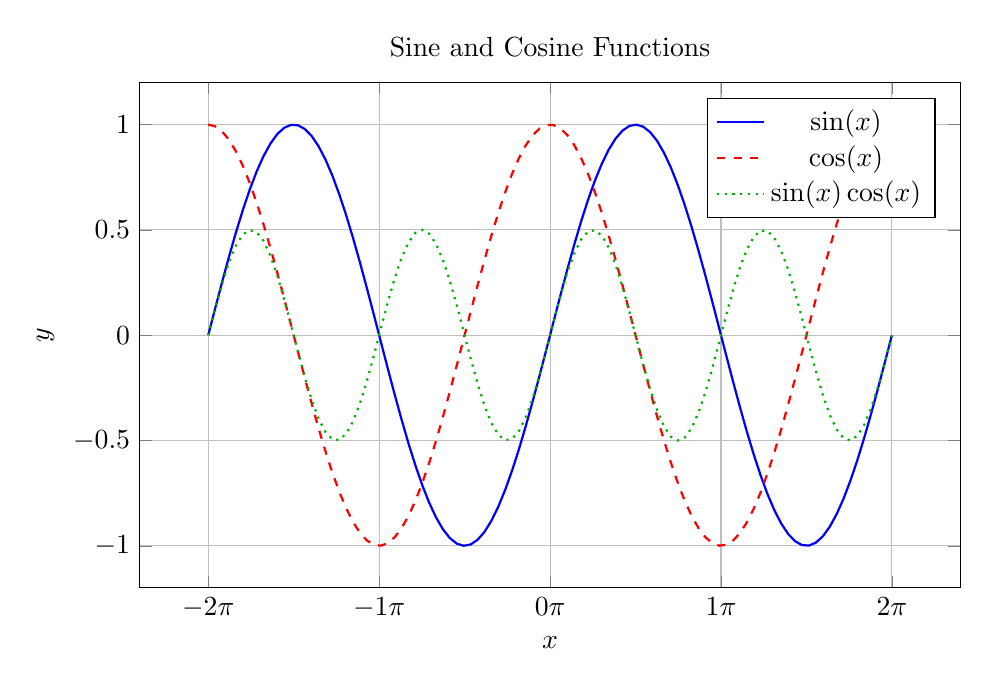
\begin{tikzpicture}
\begin{axis}[
    width=12cm,
    height=8cm,
    xlabel={$x$},
    ylabel={$y$},
    title={Sine and Cosine Functions},
    domain=-2*pi:2*pi,
    samples=100,
    grid=major,
    legend pos=north east,
    xticklabel={\pgfmathparse{\tick/pi}\pgfmathprintnumber{\pgfmathresult}$\pi$},
    xtick={-6.28318, -3.14159, 0, 3.14159, 6.28318}
]
    \addplot[blue, thick] {sin(deg(x))};
    \addlegendentry{$\sin(x)$}

    \addplot[red, thick, dashed] {cos(deg(x))};
    \addlegendentry{$\cos(x)$}

    \addplot[green!70!black, thick, dotted] {sin(deg(x))*cos(deg(x))};
    \addlegendentry{$\sin(x)\cos(x)$}
\end{axis}
\end{tikzpicture}
\end{center}

\subsection{Exponential and Logarithmic Functions}

\begin{center}
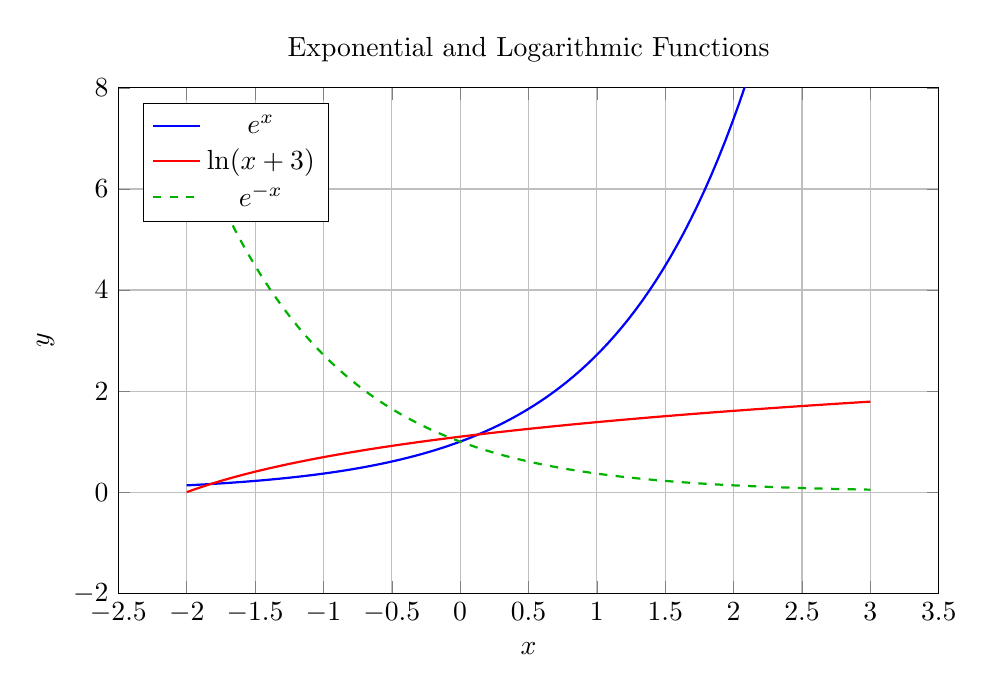
\begin{tikzpicture}
\begin{axis}[
    width=12cm,
    height=8cm,
    xlabel={$x$},
    ylabel={$y$},
    title={Exponential and Logarithmic Functions},
    domain=-2:3,
    samples=100,
    grid=major,
    legend pos=north west,
    ymin=-2,
    ymax=8
]
    \addplot[blue, thick] {exp(x)};
    \addlegendentry{$e^x$}

    \addplot[red, thick] {ln(x+3)};
    \addlegendentry{$\ln(x+3)$}

    \addplot[green!70!black, thick, dashed] {exp(-x)};
    \addlegendentry{$e^{-x}$}
\end{axis}
\end{tikzpicture}
\end{center}

\subsection{Polynomial Functions}

\begin{center}
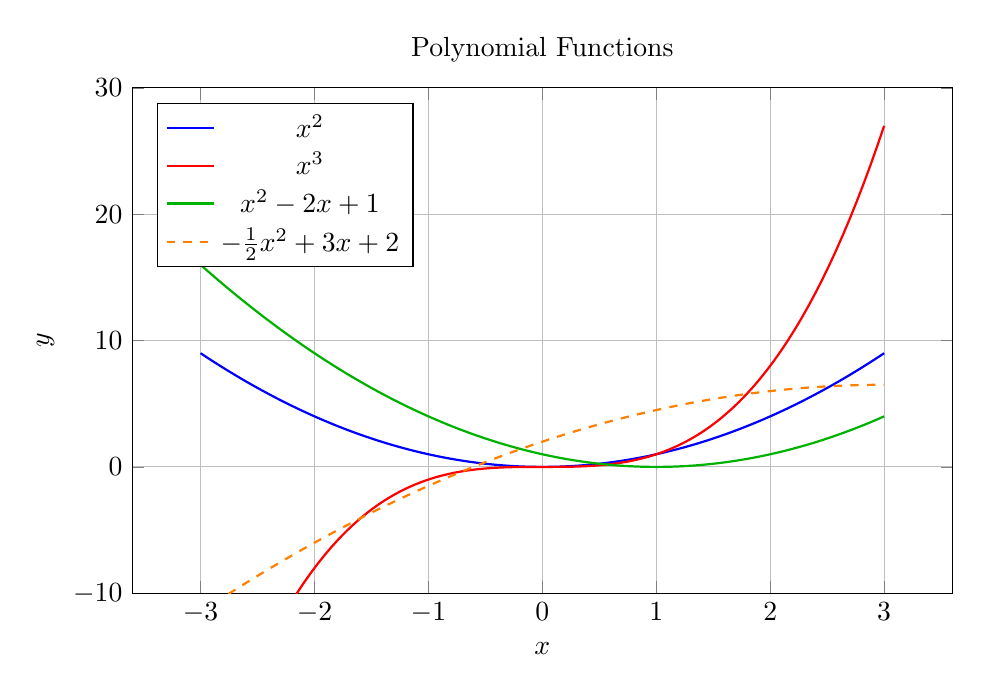
\begin{tikzpicture}
\begin{axis}[
    width=12cm,
    height=8cm,
    xlabel={$x$},
    ylabel={$y$},
    title={Polynomial Functions},
    domain=-3:3,
    samples=100,
    grid=major,
    legend pos=north west,
    ymin=-10,
    ymax=30
]
    \addplot[blue, thick] {x^2};
    \addlegendentry{$x^2$}

    \addplot[red, thick] {x^3};
    \addlegendentry{$x^3$}

    \addplot[green!70!black, thick] {x^2 - 2*x + 1};
    \addlegendentry{$x^2 - 2x + 1$}

    \addplot[orange, thick, dashed] {-0.5*x^2 + 3*x + 2};
    \addlegendentry{$-\frac{1}{2}x^2 + 3x + 2$}
\end{axis}
\end{tikzpicture}
\end{center}

\section{Parametric Plots}

\subsection{Parametric Curves}

\begin{center}
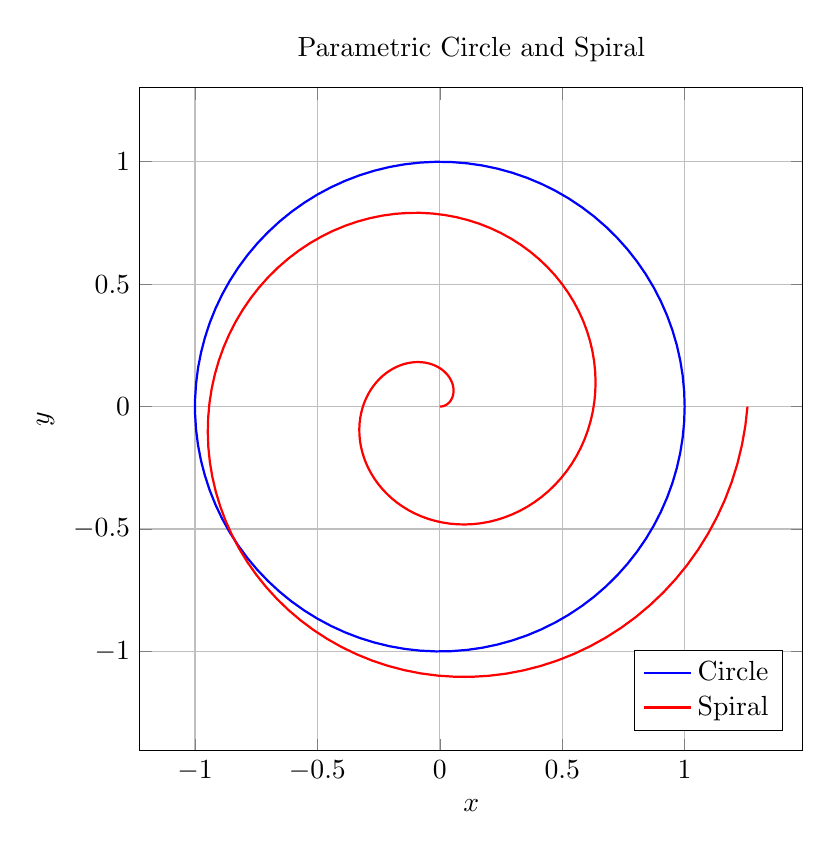
\begin{tikzpicture}
\begin{axis}[
    width=10cm,
    height=10cm,
    xlabel={$x$},
    ylabel={$y$},
    title={Parametric Circle and Spiral},
    grid=major,
    legend pos=south east,
    axis equal
]
    % Circle
    \addplot[blue, thick, domain=0:2*pi, samples=100] ({cos(deg(x))}, {sin(deg(x))});
    \addlegendentry{Circle}

    % Spiral
    \addplot[red, thick, domain=0:4*pi, samples=200] ({x*cos(deg(x))/10}, {x*sin(deg(x))/10});
    \addlegendentry{Spiral}
\end{axis}
\end{tikzpicture}
\end{center}

\section{Scatter Plots}

\subsection{Random Data Scatter}

\begin{center}
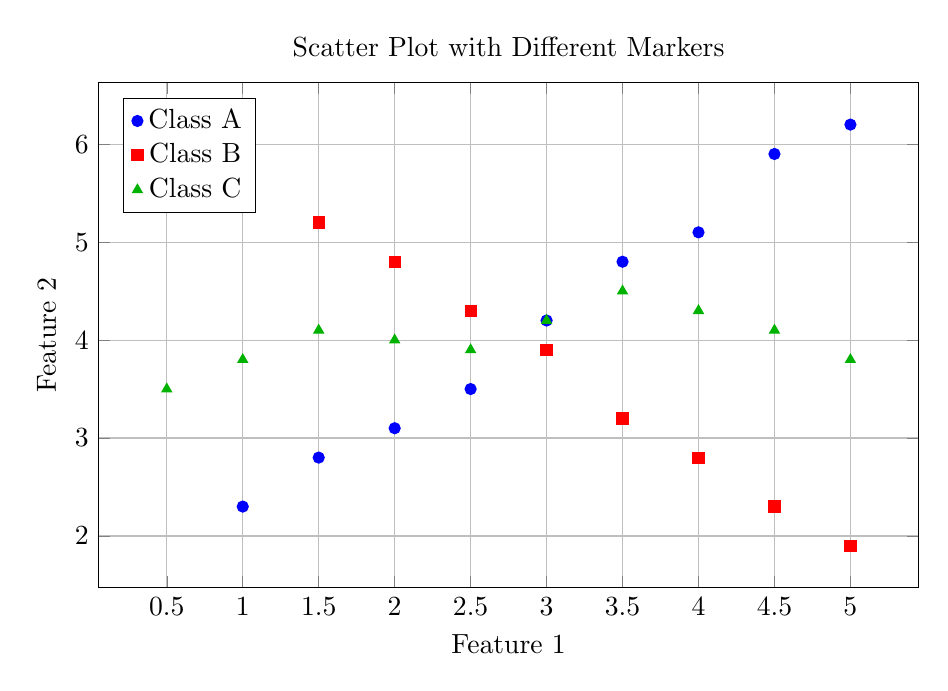
\begin{tikzpicture}
\begin{axis}[
    width=12cm,
    height=8cm,
    xlabel={Feature 1},
    ylabel={Feature 2},
    title={Scatter Plot with Different Markers},
    grid=major,
    legend pos=north west
]
    % Dataset 1
    \addplot[only marks, mark=*, blue] coordinates {
        (1, 2.3) (1.5, 2.8) (2, 3.1) (2.5, 3.5) (3, 4.2)
        (3.5, 4.8) (4, 5.1) (4.5, 5.9) (5, 6.2)
    };
    \addlegendentry{Class A}

    % Dataset 2
    \addplot[only marks, mark=square*, red] coordinates {
        (1, 5.5) (1.5, 5.2) (2, 4.8) (2.5, 4.3) (3, 3.9)
        (3.5, 3.2) (4, 2.8) (4.5, 2.3) (5, 1.9)
    };
    \addlegendentry{Class B}

    % Dataset 3
    \addplot[only marks, mark=triangle*, green!70!black] coordinates {
        (0.5, 3.5) (1, 3.8) (1.5, 4.1) (2, 4.0) (2.5, 3.9)
        (3, 4.2) (3.5, 4.5) (4, 4.3) (4.5, 4.1) (5, 3.8)
    };
    \addlegendentry{Class C}
\end{axis}
\end{tikzpicture}
\end{center}

\section{Bar Charts}

\subsection{Simple Bar Chart}

\begin{center}
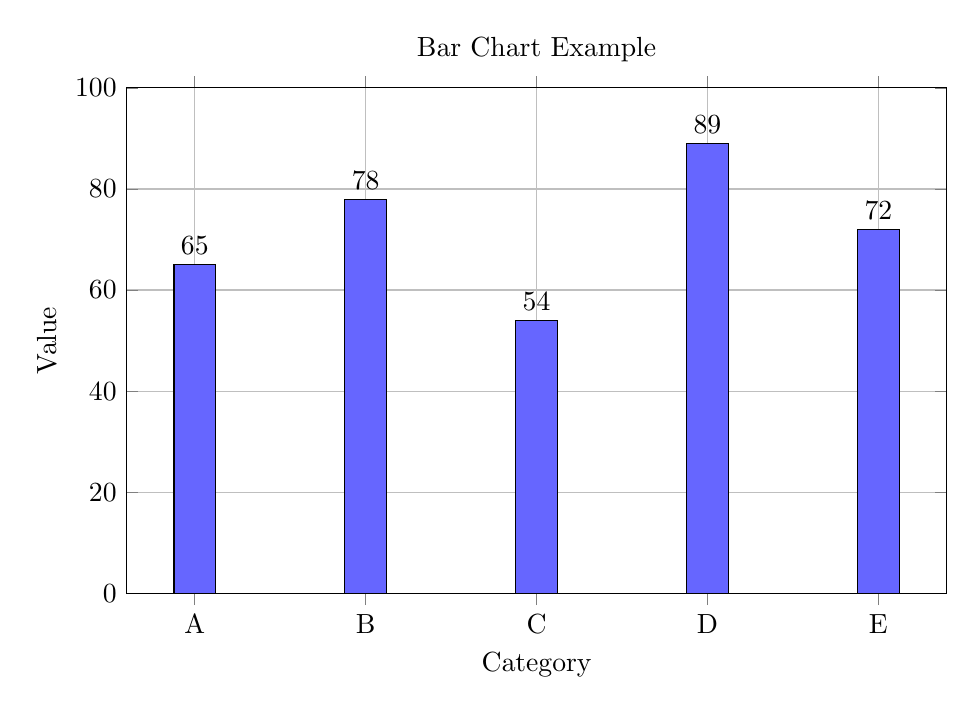
\begin{tikzpicture}
\begin{axis}[
    width=12cm,
    height=8cm,
    ybar,
    bar width=15pt,
    xlabel={Category},
    ylabel={Value},
    title={Bar Chart Example},
    symbolic x coords={A, B, C, D, E},
    xtick=data,
    nodes near coords,
    nodes near coords align={vertical},
    ymin=0,
    ymax=100,
    grid=major
]
    \addplot[fill=blue!60] coordinates {(A,65) (B,78) (C,54) (D,89) (E,72)};
\end{axis}
\end{tikzpicture}
\end{center}

\subsection{Grouped Bar Chart}

\begin{center}
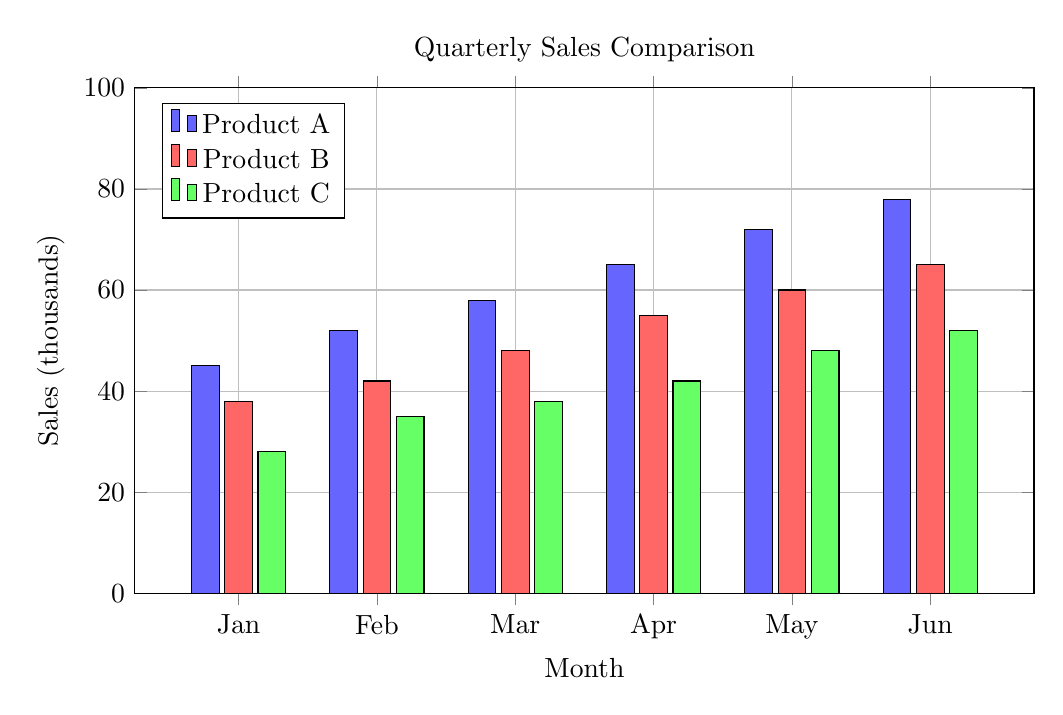
\begin{tikzpicture}
\begin{axis}[
    width=13cm,
    height=8cm,
    ybar,
    bar width=10pt,
    xlabel={Month},
    ylabel={Sales (thousands)},
    title={Quarterly Sales Comparison},
    symbolic x coords={Jan, Feb, Mar, Apr, May, Jun},
    xtick=data,
    legend pos=north west,
    ymin=0,
    ymax=100,
    grid=major,
    enlarge x limits=0.15
]
    \addplot[fill=blue!60] coordinates {
        (Jan,45) (Feb,52) (Mar,58) (Apr,65) (May,72) (Jun,78)
    };
    \addlegendentry{Product A}

    \addplot[fill=red!60] coordinates {
        (Jan,38) (Feb,42) (Mar,48) (Apr,55) (May,60) (Jun,65)
    };
    \addlegendentry{Product B}

    \addplot[fill=green!60] coordinates {
        (Jan,28) (Feb,35) (Mar,38) (Apr,42) (May,48) (Jun,52)
    };
    \addlegendentry{Product C}
\end{axis}
\end{tikzpicture}
\end{center}

\subsection{Horizontal Bar Chart}

\begin{center}
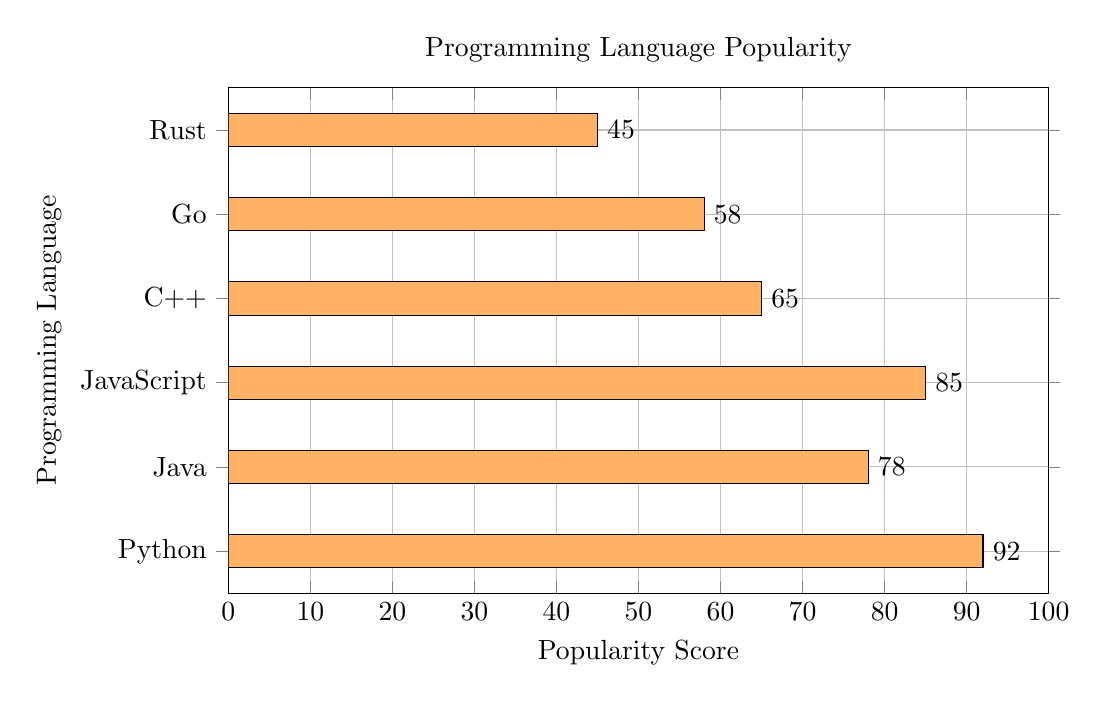
\begin{tikzpicture}
\begin{axis}[
    width=12cm,
    height=8cm,
    xbar,
    bar width=12pt,
    ylabel={Programming Language},
    xlabel={Popularity Score},
    title={Programming Language Popularity},
    symbolic y coords={Python, Java, JavaScript, C++, Go, Rust},
    ytick=data,
    nodes near coords,
    nodes near coords align={horizontal},
    xmin=0,
    xmax=100,
    grid=major
]
    \addplot[fill=orange!60] coordinates {
        (92,Python) (78,Java) (85,JavaScript) (65,C++) (58,Go) (45,Rust)
    };
\end{axis}
\end{tikzpicture}
\end{center}

\section{Advanced Plots}

\subsection{Multiple Y-Axes}

\begin{center}
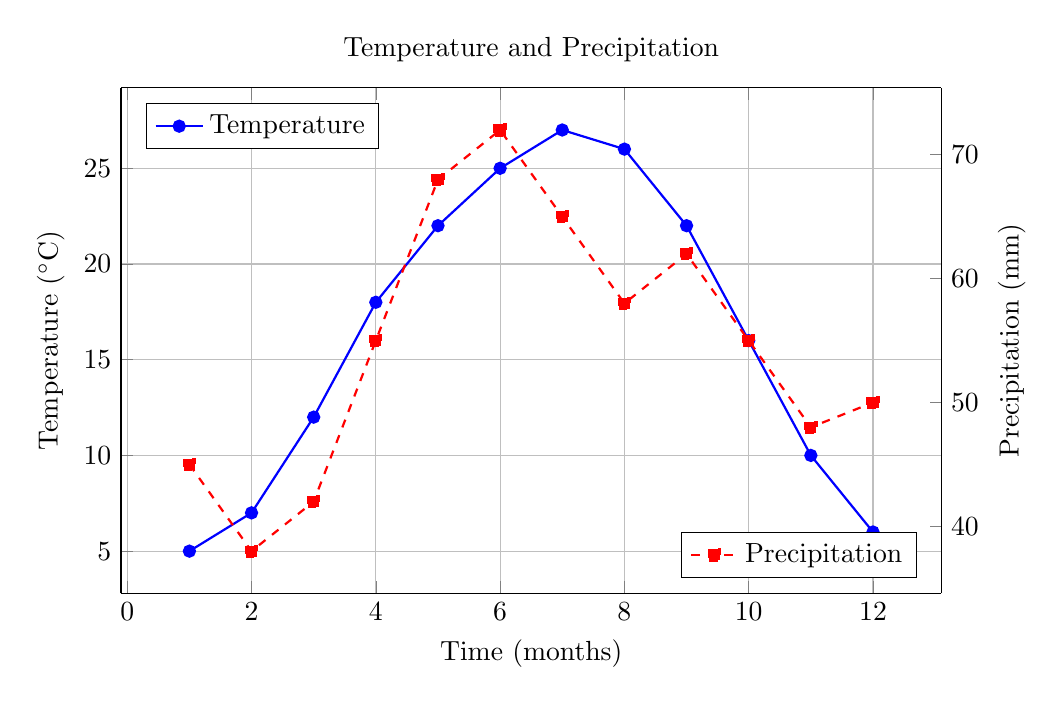
\begin{tikzpicture}
\begin{axis}[
    width=12cm,
    height=8cm,
    xlabel={Time (months)},
    ylabel={Temperature ($^\circ$C)},
    title={Temperature and Precipitation},
    axis y line*=left,
    grid=major,
    legend pos=north west
]
    \addplot[blue, thick, mark=*] coordinates {
        (1,5) (2,7) (3,12) (4,18) (5,22) (6,25) (7,27)
        (8,26) (9,22) (10,16) (11,10) (12,6)
    };
    \addlegendentry{Temperature}
\end{axis}

\begin{axis}[
    width=12cm,
    height=8cm,
    ylabel={Precipitation (mm)},
    axis y line*=right,
    axis x line=none,
    legend pos=south east
]
    \addplot[red, thick, dashed, mark=square*] coordinates {
        (1,45) (2,38) (3,42) (4,55) (5,68) (6,72) (7,65)
        (8,58) (9,62) (10,55) (11,48) (12,50)
    };
    \addlegendentry{Precipitation}
\end{axis}
\end{tikzpicture}
\end{center}

\subsection{3D Surface Plot}

\begin{center}
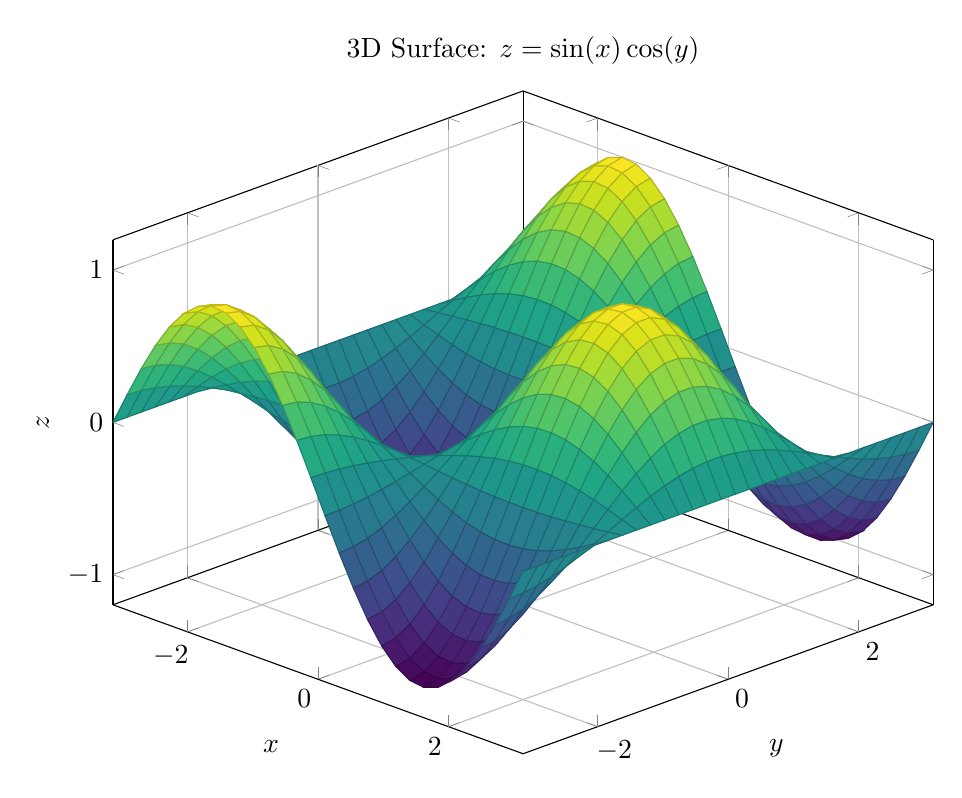
\begin{tikzpicture}
\begin{axis}[
    width=12cm,
    height=10cm,
    view={45}{30},
    xlabel={$x$},
    ylabel={$y$},
    zlabel={$z$},
    title={3D Surface: $z = \sin(x)\cos(y)$},
    colormap/viridis,
    grid=major
]
    \addplot3[
        surf,
        samples=30,
        domain=-pi:pi
    ]
    {sin(deg(x))*cos(deg(y))};
\end{axis}
\end{tikzpicture}
\end{center}

\subsection{Contour Plot}

\begin{center}
\begin{tikzpicture}
\begin{axis}[
    width=10cm,
    height=10cm,
    xlabel={$x$},
    ylabel={$y$},
    title={Contour Plot: $z = x^2 + y^2$},
    view={0}{90},
    colormap/hot,
    colorbar
]
    \addplot3[
        contour gnuplot={number=15},
        samples=50,
        domain=-2:2
    ]
    {x^2 + y^2};
\end{axis}
\end{tikzpicture}
\end{center}

\section{Compilation Notes}

To compile this document:
\begin{verbatim}
pdflatex --shell-escape pgfplots_demo.tex
\end{verbatim}

The \texttt{--shell-escape} flag is required for certain plot types (like contour plots)
that use external programs.

\end{document}
